برای فرمول
$\neg p_3\vee (p_1\to p_3)$
یک دنبالهٔ ساختمان بنویسید و درخت تجزیهٔ آن را رسم کنید.
%ANS tree needs editing
\begin{ans}
    دنباله ساختمان: 
    \begin{flushleft}
        $p_1,p_3,\neg p_3,p_1\to p_3,\neg p_3\vee (p_1\to p_3)$
    \end{flushleft}
    درخت تجزیه:
    \begin{flushleft}
        
        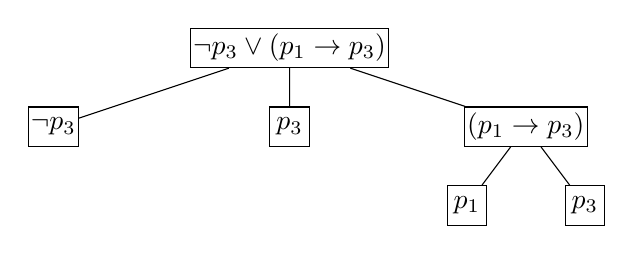
\begin{tikzpicture}
            [level distance=10mm,
            every node/.style={draw=black, inner sep=1pt, minimum size=5mm},
            level 1/.style={sibling distance=30mm},
            level 2/.style={sibling distance=15mm},
            level 3/.style={sibling distance=8mm}]
            \node {$\neg p_3 \vee (p_1 \to p_3)$}
            child { node {$\neg p_3$} }
                child{ node {$p_3$}}
            child { node {$(p_1 \to p_3)$}
                child { node {$p_1$} }
                child { node {$p_3$} }
            };
            ]
        \end{tikzpicture}
    \end{flushleft}
\end{ans}
